\chapter{Kerr-Schild metrics}
\label{s:ksm}

\minitoc

\section{Generic Kerr-Schild spacetimes}

\subsection{Definition} \label{s:ksm:def_Kerr_Schild}

A spacetime $(\M,\w{g})$ is said to have a
\defin{Kerr-Schild metric}\index{Kerr-Schild!metric} iff the metric tensor $\w{g}$
can be written
\be \label{e:ksm:g_KerrSchild}
   \encadre{ \w{g} = \w{f} + 2 H \uu{k}\otimes\uu{k} },
\ee
or equivalently (in index notation):
\be \label{e:ksm:g_KerrSchild_comp}
    \encadre{ g_{\alpha\beta} = f_{\alpha\beta} + 2 H k_\alpha k_\beta },
\ee
where $\w{f}$ is a flat Lorentzian metric on $\M$ (Minkowski metric),
$H$ is a scalar field on $\M$ and $\uu{k}$ is a 1-form on $\M$ such that the
vector associated to it via $\w{f}$ is a null vector of the metric
$\w{f}$:
\be
     f^{\mu\nu} k_\mu k_\nu = 0 ,
\ee
where $f^{\mu\nu}$ stands for the components of the inverse of the metric
$\w{f}$ (i.e. $f^{\alpha\mu} f_{\mu\beta} = \delta^\alpha_{\ \; \beta}$).

A motivation for studying
Kerr-Schild metrics is that the inverse metric has a simple expression:
\be \label{e:ksm:g_inverse}
    g^{\alpha\beta} = f^{\alpha\beta} - 2 H k^\alpha k^\beta ,
\ee
where
\be \label{e:ksm:k_up_comp}
    k^\alpha := f^{\alpha\mu} k_\mu .
\ee
\emph{Proof:} we have successively:
\bea
   (f^{\alpha\mu} - 2 H k^\alpha k^\mu) g_{\mu\beta} & = &
   (f^{\alpha\mu} - 2 H k^\alpha k^\mu) (f_{\mu\beta} + 2 H k_\mu k_\beta) \nonumber \\
   & = & \underbrace{f^{\alpha\mu} f_{\mu\beta}}_{\delta^\alpha_{\ \; \beta}}
    + 2 H \underbrace{f^{\alpha\mu} k_\mu}_{k^\alpha} k_\beta
    - 2 H k^\alpha \underbrace{k^\mu f_{\mu\beta}}_{k_\beta}
    - 4 H^2 k^\alpha \underbrace{k^\mu k_\mu}_{0} k_\beta \nonumber \\
   & = & \delta^\alpha_{\ \; \beta} , \nonumber
\eea
which establishes Eq.~\eqref{e:ksm:g_inverse}. \qed

Given (\ref{e:ksm:g_inverse}), it is easy to see that the vector field
$\w{k}$ associated
to the 1-form $\uu{k}$ by $\w{g}$-duality (cf. Sec.~\ref{s:bas:metric_dual})
is the same as the vector field
obtained by $\w{f}$-duality:
\[
    g^{\alpha\mu} k_\mu = (f^{\alpha\mu} - 2 H k^\alpha k^\mu) k_\mu
                        = \underbrace{f^{\alpha\mu} k_\mu}_{k^\alpha}
                          - 2H k^\alpha \underbrace{k^\mu k_\mu}_{0}
                        = k^\alpha .
\]
Accordingly, we may write the components of $\w{k}$ simply as $k^\alpha$
without having to specify whether the index has been raised with the
metric $\w{g}$ or with the metric $\w{f}$:
\be
    k^\alpha = f^{\alpha\mu} k_\mu  = g^{\alpha\mu} k_\mu .
\ee
It follows immediately that $\w{k}$ is a null vector field for
both metrics:
\be
   \encadre{ \w{g}(\w{k}, \w{k}) = \w{f}(\w{k}, \w{k}) = 0 }.
\ee


If $(\M,\w{g})$ is a spacetime of Kerr-Schild type, then \defin{Kerr-Schild
coordinates}\index{Kerr-Schild!coordinates}
are coordinates $(x^\alpha) = (t,x,y,z)$ that are Minkowskian\index{Minkowskian!coordinates}
for $\w{f}$, i.e. coordinates in which the components of the flat metric
$\w{f}$ take the form
\be \label{e:ksm:ds_eta}
    f_{\mu\nu} \, \D x^\mu \, \D x^\nu = - \D t^2 + \D x^2 + \D y^2
        + \D z^2 .
\ee

\subsection{Basic property}

\begin{greybox}
Let $\w{g}$ be a Kerr-Schild metric.
If $\w{g}$ obeys the vacuum Einstein
equation\index{Einstein!equation}, i.e. if the Ricci tensor of $\w{g}$ vanishes identically:
\be
    R_{\alpha\beta} = 0 ,
\ee
then the scalar field $H$ appearing in Eq.~(\ref{e:ksm:g_KerrSchild})
can be chosen so that $\w{k}$ is a geodesic vector field\footnote{See Sec.~\ref{s:geo:gener_param} for the definition of a geodesic vector field.}:
\be \label{e:ksm:k_geodesic}
    \encadre{ k^\mu \nabla_\mu k^\alpha = 0 },
\ee
where $\nabla$ stands for the covariant derivative associated with $\w{g}$.
\end{greybox}

The proof of the above proposition can be found in Ref.~\cite{KerrS65}.


%%%%%%%%%%%%%%%%%%%%%%%%%%%%%%%%%%%%%%%%%%%%%%%%%%%%%%%%%%%%%%%%%%%%%%%%%%%%%%%

\section{Case of Kerr spacetime}

\subsection{Kerr-Schild form}

Let consider the Kerr spacetime $(\M,\w{g})$, where $\M$ is the manifold
(\ref{e:ker:def_M_Kerr_spacetime}): $\M = \R^2\times\SS^2 \setminus \ring$
and $\w{g}$ is the metric tensor given by Eq.~(\ref{e:ker:metric_Kerr_3p1})
in terms of the 3+1 Kerr coordinates $(\ti, r, \th,\tph)$ introduced in
Sec.~\ref{s:ker:3p1_Kerr_coord}.
Let us show that $\w{g}$ is a Kerr-Schild metric, with the associated null vector
field $\w{k}$ being nothing but the vector field generating the principal
ingoing null geodesics $\Li^{\rm in}_{(v,\th,\tph)}$  discussed in Sec.~\ref{s:ker:principal_geod}.
Its expression in terms of the 3+1 Kerr coordinates is given by Eq.~(\ref{e:ker:k_ti_tr}):
\be \label{e:ksm:k_Kerr}
    \encadre{ \w{k} = \wpar_\ti - \wpar_{\tilde r} }.
\ee
In other words, the components of $\w{k}$ with respect to the 3+1 Kerr coordinates $(\ti, r, \th,\tph)$ are $k^\alpha = (1, -1, 0, 0)$.
The 1-form $\uu{k}$ associated to $\w{k}$ by $\w{g}$-duality is easily computed
from $k_\alpha = g_{\alpha\mu} k^\mu$, with $g_{\alpha\mu}$ given by
Eq.~(\ref{e:ker:metric_Kerr_3p1}). We get
$k_\alpha = (-1, -1, 0, a\sin^2\th)$, i.e.
\be \label{e:ksm:k_form_Kerr}
    \uu{k} = - \dd \ti - \dd r + a\sin^2\th \, \dd\tph .
\ee
Let us then introduce the symmetric bilinear form
\be
    \w{f} := \w{g} - 2 H \uu{k} \otimes \uu{k} ,
\ee
where $H$ is the following scalar field on $\M$:
\be \label{e:ksm:H_Kerr}
   \encadre{ H := \frac{m r}{\rho^2} },
\ee
with $\rho^2 := r^2 + a^2 \cos^2\th$ [Eq.~(\ref{e:ker:def_rho2})].
The expression of $\w{f}$ in terms of the 3+1 Kerr coordinates is deduced
from that of $\w{g}$ [Eq.~(\ref{e:ker:metric_Kerr_3p1})] and that of
$\uu{k}$ [Eq.~(\ref{e:ksm:k_form_Kerr})]:
\be \label{e:ksm:f_Kerr}
  \encadre{  f_{\mu\nu}\,  \D x^\mu \D x^\nu = - \D\ti^2 + \D r^2 - 2 a \sin^2\th \, \D r \, \D\tph
    + \rho^2\, \D \th^2 + (r^2 + a^2)\sin^2\th\, \D \tph^2 }.
\ee
It is easy to check that $f^{\alpha\beta} := g^{\alpha\beta} + 2 H k^\alpha k^\beta$
defines an inverse of $\w{f}$: $f^{\alpha\mu} f_{\mu\beta} = \delta^\alpha_{\ \; \beta}$
(computation similar to that in Sec.~\ref{s:ksm:def_Kerr_Schild}). Hence the
symmetric bilinear form $\w{f}$ is nondegenerate; this implies that $\w{f}$
is a \emph{metric tensor} on $\M$ (cf. Sec.~\ref{s:bas:metric}).
Given the components (\ref{e:ksm:k_form_Kerr}), it is immediate to check that $\w{k}$ is a null vector for $\w{f}$ as well: $\w{f}(\w{k}, \w{k}) = 0$.
Moreover, $\w{f}$ is a \emph{flat} metric, since a direct computation of its
Riemann tensor (cf. the notebook \ref{s:sam:Kerr_Schild}) reveals that
\be
    \mathrm{\bf Riem}(\w{f}) = 0 .
\ee
In view of the definition given in Sec.~\ref{s:ksm:def_Kerr_Schild},
we conclude that
\begin{greybox}
The Kerr metric $\w{g}$ is a Kerr-Schild metric, i.e. it can be written in
the form (\ref{e:ksm:g_KerrSchild}) with the flat metric
$\w{f}$ given by Eq.~(\ref{e:ksm:f_Kerr}), the scalar field $H$ given
by Eq.~(\ref{e:ksm:H_Kerr}) and the null vector $\w{k}$ given by
Eq.~(\ref{e:ksm:k_Kerr}), $\w{k}$ being the tangent vector field to
the principal ingoing null geodesics.
\end{greybox}
In Sec.~\ref{s:ker:principal_geod},
we have already noticed that $\w{k}$ is a geodesic vector:
$\wnab_{\w{k}}\, \w{k} = 0$ [Eq.~(\ref{e:ker:nab_k_k})], in agreement with
(\ref{e:ksm:k_geodesic}).

\begin{remark}
The Kerr metric can also be brought to the Kerr-Schild form by using the
tangent vector field to the principal \emph{outgoing} null geodesics. Hence
the Kerr-Schild decomposition (\ref{e:ksm:g_KerrSchild}) is not unique for
the Kerr metric.
\end{remark}

\subsection{Kerr-Schild coordinates on Kerr spacetime}

It is not immediately obvious that the metric $\w{f}$ given by
Eq.~(\ref{e:ksm:f_Kerr}) is a flat Lorentzian metric.
Let us introduce coordinates in which $\w{f}$ takes a manifestly Minkowskian
form, i.e. Kerr-Schild coordinates, according to the nomenclature introduced
in Sec.~\ref{s:ksm:def_Kerr_Schild}.

Actually, if $a\not=0$, one cannot introduce a Kerr-Schild coordinate system on the whole
spacetime manifold $\M = \R^2\times\SS^2 \setminus \ring$ as defined by
Eq.~(\ref{e:ker:def_M_Kerr_spacetime}). One has to split it in two parts:
\begin{subequations}
\begin{align}
    \M & :=  \M_+ \cup \M_- , \\
    \M_+ & :=  \R\times {[0,+\infty)}\times\SS^2 \setminus \ring\\
    \M_- & :=  \R\times {(-\infty,0]}\times\SS^2 \setminus \ring .
\end{align}
\end{subequations}
In other words, $\M_+$ is the part $r\geq 0$ of $\M$ and $\M_-$ is the part
$r\leq 0$. Note that $\M_+$ and $\M_-$ overlap at $r=0$ and that in terms of the domains introduced in Sec.~\ref{s:ker:expr_BL},
$\M_+$ contains $\M_{\rm I}$, $\M_{\rm II}$ and a part of $\M_{\rm III}$,
while $\M_-$ is entirely included in $\M_{\rm III}$.
The \defin{Kerr-Schild coordinates} $(\ti, x, y, z)$
of $\M_+$ are defined from the 3+1 Kerr coordinates
$(\ti, r, \th,\tph)$ by the formulas:
\begin{subequations}
\label{e:ksm:K_to_KS}
\bea
    \ti & = & \ti \\
    x & = & (r\cos\tph - a \sin\tph) \sin \th  \label{e:ksm:x_Kerr}\\
    y & = & (r\sin\tph + a \cos\tph) \sin \th  \label{e:ksm:y_Kerr}\\
    z & = & r\cos \th . \label{e:ksm:z_Kerr}
\eea
\end{subequations}
\begin{remark}
For $a=0$, Eqs.~\eqref{e:ksm:x_Kerr}-\eqref{e:ksm:z_Kerr} reduce to the standard
relations between Cartesian and spherical coordinates in Euclidean space.
\end{remark}
\begin{remark}
Equations~(\ref{e:ksm:x_Kerr})-(\ref{e:ksm:y_Kerr}) can be combined into a single
relation:
\be
    x + i y = (r + i a) \mathrm{e}^{i\tph} \sin\th .
\ee
\end{remark}
From Eqs.~(\ref{e:ksm:x_Kerr})-(\ref{e:ksm:y_Kerr}), we
get
\be
    x^2 + y^2 = (r^2 + a^2)\sin^2\th .
\ee
Combining with Eq.~(\ref{e:ksm:z_Kerr}) yields:
\be \label{e:ksm:ellipsoids}
\encadre{ \frac{x^2 + y^2}{r^2 + a^2} + \frac{z^2}{r^2} = 1 } .
\ee
This is a quadratic equation in $r^2$. Solving it results in
\be \label{e:ksm:r_xyz}
    r = \sqrt{ \frac{1}{2} \left(
        x^2 + y^2 + z^2 - a^2 +
        \sqrt{(x^2 + y^2 + z^2 - a^2)^2 + 4 a^2 z^2} \right)}  .
\ee
A direct computation via the tensor change of components formula with
the transformation (\ref{e:ksm:K_to_KS}) yields to
the following components of $\w{f}$ in terms on the coordinates
$(x^\alpha)=(\ti, x, y, z)$
(cf. the notebook \ref{s:sam:Kerr_Schild}):
\be \label{e:ksm:f_Kerr_KS}
 f_{\mu\nu}\,  \D x^\mu \D x^\nu = - \D\ti^2 + \D x^2 + \D y^2 + \D z^2 ,
\ee
which proves that $(\ti, x, y, z)$ are Kerr-Schild coordinates, as announced.

The expression of the vector $\w{k}$ in terms of the Kerr-Schild coordinates
is obtained similarly:
\be
    \w{k} = \wpar_{\ti} - \frac{r x + a y}{r^2 + a^2} \, \wpar_x
        - \frac{r y - a x}{r^2 + a^2} \, \wpar_y
        - \frac{z}{r}\, \wpar_z .
\ee
In this formula, $r$ is to be considered as the function of $(x,y,z)$ given
by Eq.~(\ref{e:ksm:r_xyz}). For the associated 1-form, we get
\be \label{e:ksm:k_form_Kerr_KS}
    \uu{k} = - \dd\ti - \frac{r x + a y}{r^2 + a^2} \, \dd x
       - \frac{r y - a x}{r^2 + a^2} \, \dd y
        - \frac{z}{r}\, \dd z .
\ee
The scalar factor $H$ can be re-expressed from Eq.~(\ref{e:ksm:H_Kerr})
in terms of $z$ and $r$:
\be \label{e:ksm:H_Kerr_zr}
    H = \frac{m r^3}{r^4 + a^2 z^2}  .
\ee

\begin{remark}
If $a=0$ (Schwarzschild limit), we get
\be \label{e:ksm:lim_a_zero}
    r = \sqrt{x^2 + y^2 + z^2}, \quad
    H = \frac{m}{r} \quad\mbox{and}\quad
    \uu{k} = - \dd\ti - \frac{x}{r} \, \dd x
       - \frac{y}{r} \, \dd y
        - \frac{z}{r}\, \dd z .
\ee
\end{remark}

\begin{remark}
For $a \not = 0$, the relations (\ref{e:ksm:lim_a_zero}) hold at first order
in the limit $r \gg a$, or equivalently in the limit $\sqrt{x^2 + y^2 + z^2} \gg a$.
\end{remark}

The explicit form of the components
$g_{\mu\nu}$ of the Kerr metric in Kerr-Schild coordinates can be read off by expanding the line
element
\be \label{e:ksm:g_comp_KS}
\encadre{ \begin{array}{ll}
g_{\mu\nu} \, \D x^\mu \, \D x^\nu = & - \D \ti^2 + \D x^2 + \D y^2
        + \D z^2 \\
        &\displaystyle  + \frac{2m r^3}{r^4 + a^2 z^2} \left( \D \ti
        + \frac{r x + a y}{r^2 + a^2} \, \D x
        + \frac{r y - a x}{r^2 + a^2} \, \D y + \frac{z}{r} \, \D z \right) ^2
\end{array} } ,
\ee
which is obtained by combining Eqs~(\ref{e:ksm:g_KerrSchild_comp}), (\ref{e:ksm:f_Kerr_KS}),
(\ref{e:ksm:H_Kerr_zr})
and (\ref{e:ksm:k_form_Kerr_KS}).
\begin{remark}
It is clear on \eqref{e:ksm:g_comp_KS} that all metric components in Kerr-Schild
coordinates are regular at the event horizon, which is defined by $r= m + \sqrt{m^2-a^2}$.
This property, which is shared by the 3+1 Kerr coordinates,
is in sharp contrast with the metric components in the standard
Boyer-Lindquist coordinates [cf. Eq.~(\ref{e:ker:metric_BL})].
\end{remark}


On the domain $\M_-$, i.e. for $r\leq 0$,
one has to introduce another patch of Kerr-Schild coordinates, $(\ti,x',y',z')$ say,
such that
\be
    r := - \sqrt{ \frac{1}{2} \left(
        {x'}^2 + {y'}^2 + {z'}^2 - a^2 +
        \sqrt{({x'}^2 + {y'}^2 + {z'}^2 - a^2)^2 + 4 a^2 {z'}^2} \right)} .
\ee

\begin{figure}
\centerline{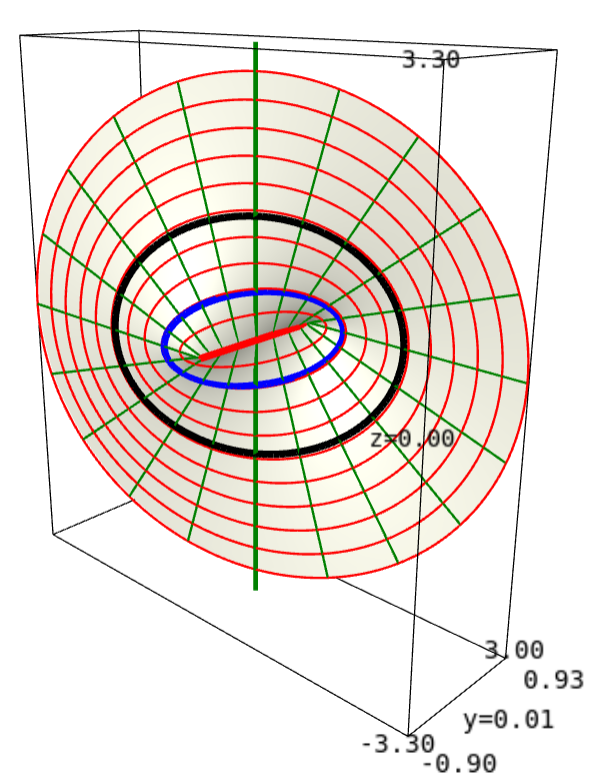
\includegraphics[width=0.45\textwidth]{ksm_phi_cut.png}}
\caption[]{\label{f:ksm:phi_cut} \footnotesize
Surface $\ti=\mathrm{const}$ and $\tph\in\{0,\pi\}$ of the $a=0.9\, m$
Kerr spacetime
depicted in terms of
the Kerr-Schild coordinates $(x,y,z)$. The vertical thick green line is
the axis of rotation. On the right of it $\tph=0$, while on the left
of it $\tph=\pi$.
The red lines are curves $r=\mathrm{const}$,
while the green ones are curves $\th=\mathrm{const}$. The thick black curve corresponds
to the black hole event horizon and the thick blue curve to the Cauchy horizon
(cf. Sec.~\ref{s:ker:Cauchy_hor}). The thick red segment in the plane $z=0$
marks the intersection of the surface with the disk $r=0$.
\textsl{[Figure produced with the notebook \ref{s:sam:Kerr_Schild}]}
}
\end{figure}

\begin{figure}
\centerline{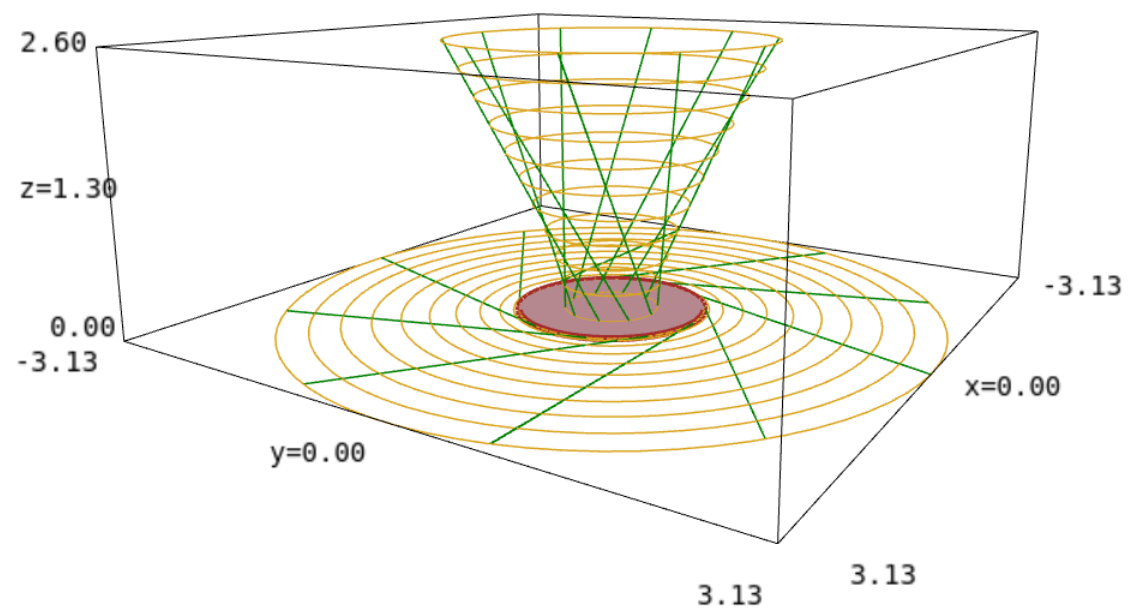
\includegraphics[width=0.7\textwidth]{ksm_theta_cut.png}}
\caption[]{\label{f:ksm:theta_cut} \footnotesize
Surfaces $(\ti,\th)=\mathrm{const}$ of
the $a=0.9\, m$ Kerr spacetime depicted in terms of
the Kerr-Schild coordinates $(x,y,z)$.
The disk-like surface in the plane $z=0$ is for $\th=\pi/2$, while
the cone-like surface is for $\th=\pi/6$.
The brown lines are curves $(r,\th)=\mathrm{const}$,
while the green ones are curves $(\th,\tph)=\mathrm{const}$.
The central pink disk is the disk $r=0$, the boundary of which is the
curvature singularity.
\textsl{[Figure produced with the notebook \ref{s:sam:Kerr_Schild}]}
}
\end{figure}

\begin{figure}
\centerline{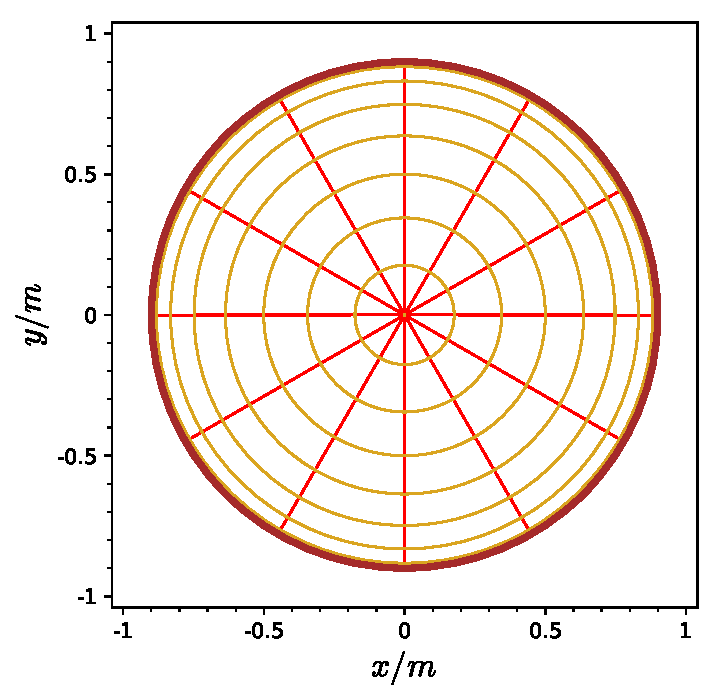
\includegraphics[width=0.45\textwidth]{ksm_rzero_disk.pdf}}
\caption[]{\label{f:ksm:rzero_disk} \footnotesize
Disk $r=0$ of the $a=0.9\, m$ Kerr spacetime depicted in terms of
the Kerr-Schild coordinates $(x,y)$.
\textsl{[Figure produced with the notebook \ref{s:sam:Kerr_Schild}]}
}
\end{figure}



The identity (\ref{e:ksm:ellipsoids}) shows that, in the Euclidean space spanned by the $(x,y,z)$ coordinates,
the surfaces of constant $r\not=0$ are
confocal\footnote{In any plane containing the axis of symmetry $x^2+y^2=0$, the trace of
the ellipsoids are ellipses that share the same foci, located
at the abscissas $\pm a$ along the $z=0$ axis.}
 ellipsoids of revolution. For $r=0$ and $a>0$, Eq.~\eqref{e:ksm:r_xyz} shows that the surface
of constant $r$ is the disk of radius $a$ centered at the origin in the plane
$z=0$:
\be \label{e:ksm:disk_r0}
    r = 0 \iff \left\{ \begin{array}{l}
        z = 0 \\
        x^2 + y^2 \leq a^2 .
        \end{array} \right.
\ee
\emph{Proof:} starting from Eq.~\eqref{e:ksm:r_xyz}, we have successively
\bea
    r = 0 & \iff & x^2 + y^2 + z^2 - a^2 =
        - \sqrt{(x^2 + y^2 + z^2 - a^2)^2 + 4 a^2 z^2} \nonumber \\
        & \iff & \begin{cases}
               (x^2 + y^2 + z^2 - a^2)^2 =   (x^2 + y^2 + z^2 - a^2)^2 + 4 a^2 z^2 \\
               x^2 + y^2 + z^2 - a^2 \leq 0
               \end{cases} \nonumber \\
        & \iff &  \begin{cases}
                  4 a^2 z^2 = 0 \\
                  x^2 + y^2 + z^2 \leq a^2,
                 \end{cases}
        \iff
        \begin{cases}
                  z = 0 \\
                  x^2 + y^2 \leq a^2,
                  \end{cases}  \nonumber
\eea
where the last equivalence assumes $a\not=0$. \qed




\subsection{Link with Boyer-Lindquist coordinates}

The link between the Kerr-Schild coordinates $(\ti,x,y,z)$ and the Boyer-Lindquist
coordinates $(t,r,\th,\ph)$
is obtained by combining Eqs.~(\ref{e:ksm:K_to_KS}) with Eqs.~(\ref{e:ker:Kerr_3p1_BL_int}).


\begin{hist}
Kerr-Schild coordinates have been introduced by Roy Kerr\index{Kerr, R.} in his famous 1963 paper
\cite{Kerr63} announcing the discovery of the
metric that bares his name; they have been discussed further by Kerr and Alfred
Schild\index{Schild, A.}
in 1965 \cite{KerrS65}, as well as by
Robert Boyer\index{Boyer, R.H.} and Richard Lindquist\index{Lindquist, R.W.}
in 1967 \cite{BoyerL67}, Brandon Carter\index{Carter, B.} in 1968
\cite{Carte68}
and Stephen Hawking\index{Hawking, S.W.} and George Ellis\index{Ellis, G.F.R} in 1973 \cite{HawkiE73}.
\end{hist}
